\documentclass[../main.tex]{subfiles}

\begin{document} %%%%%%%%%%%%%%%%%%%%%%%%%%%%%%%%%%%%%%%%%%%%%%%%%%%%%%%%%%%%
\section{Programación Orientada a Objetos} 
    \begin{definition} Paradigmas de Programación
        \begin{itemize}
            \item \textbf{Imperativos:} (énfasis en la ejecución de instrucciones)
                \begin{itemize}
                    \item Programación Procedimental (p. ej. Pascal).
                    \item Programación Orientada a Objetos (p. ej. Smalltalk, Java = multiparadigma).
                \end{itemize}
            \item \textbf{Declarativos:} (énfasis en la evaluación de expresiones)
                \begin{itemize}
                    \item Programación Funcional (p. ej. Haskell).
                    \item Programación Lógica (p. ej. Prolog).
                \end{itemize}
        \end{itemize}
    \end{definition}

    \subsection{Sistemas Orientados a Objetos}
        \begin{definition} \textbf{(Entidad)} 
            Una entidad es un objeto del mundo real que tiene un identificador único, un estado y un comportamiento \cite{def_entidad}.\\
            
            \underline{Tipos de entidades:}
            \begin{itemize}
                \item \textbf{Entidades físicas:} (p. ej. un auto, una persona, un libro).
                \item \textbf{Entidades conceptuales:} (p. ej. un viaje, una reserva, un préstamo).
                \item \textbf{Entidades fuertes:} son entidades que pueden sobrevivir por sí solas. 
                \item \textbf{Entidades debil:} no pueden existir sin una entidad fuerte y se representan con un cuadrado con doble línea
            \end{itemize}
        \end{definition}

        \begin{definition} \textbf{(Clase)}
            Una clase es un conjunto de objetos que comparten características y comportamientos comunes, así como propiedades y atributos comunes. Es un prototipo o plano definido por el usuario a partir del cual se crean objetos

            % cargamos imagen
            \begin{figure}[ht]
                \centering
                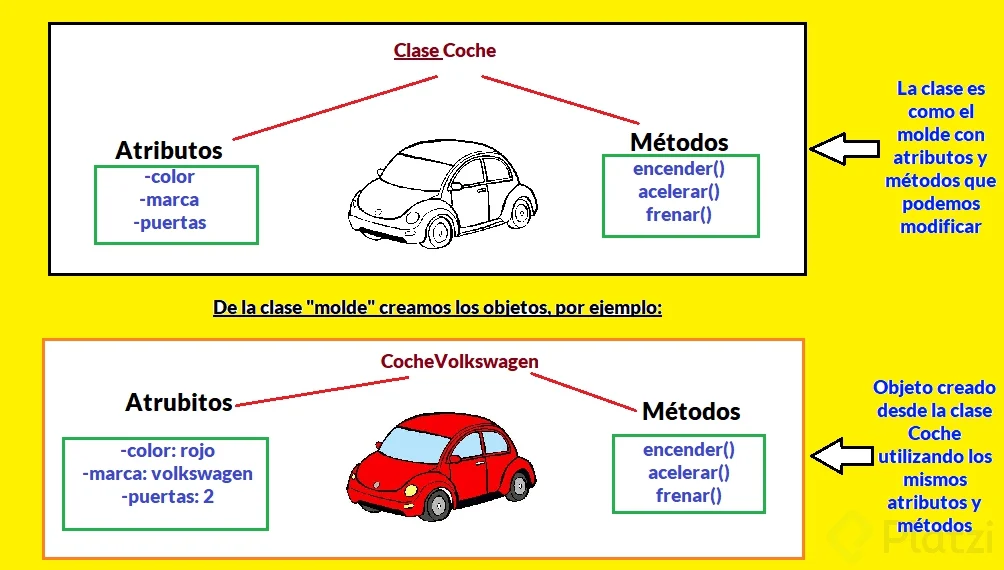
\includegraphics[width=0.9\textwidth]{../images/clase.png}
                \caption{Clase}
                \label{fig:clase_auto}
            \end{figure}

        \end{definition}

        \begin{definition} \textbf{(Objeto)}
            Un objeto es una entidad que puede recibir mensajes, responder a los mismos y enviar mensajes a otros objetos. Un objeto es una entidad que tiene comportamiento.\\

            \underline{Todo objeto tiene tres características:}
            \begin{itemize}
                \item \textbf{Identidad:} Es un identificador único que lo diferencia de los demás objetos. La identidad es lo que distingue a un objeto de otro.
                \item \textbf{Estado:} El estado es la situación en que un objeto se encuentra. Un objeto puede cambiar su estado a través del tiempo.
                \item \textbf{Comportamiento:} Es el conjunto de posibles respuestas de un objeto ante los mensajes que recibe. El comportamiento de un objeto está compuesto por las respuestas a los mensajes que recibe un objeto, que a su vez pueden provocar:
                    \begin{itemize}
                        \item Un cambio de estado en el objeto receptor del mensaje.
                        \item La devolución del estado de un objeto, en su totalidad o parcialmente
                        \item El envío de un mensaje desde el objeto receptor a otro objeto (delegación)
                    \end{itemize}
            \end{itemize}

            Cuando un objeto es creado a partir de una clase, se dice que el objeto es una \textbf{instancia} de la clase, esto se puede ver en la Figura \ref{fig:clase_auto}, creación del objeto CocheVolkswagen.
        \end{definition}

        \begin{definition} \textbf{(Atributo (o variable de instancia))}
            En POO, llamamos atributo a una variable interna del objeto que sirve para almacenar parte del estado del mismo
        \end{definition}

        \begin{definition} \textbf{(Método)}
            Llamamos método a la implementación de la respuesta de un objeto a un mensaje. En términos de implementación, se asemeja a funciones o procedimientos de programación en otros paradigmas.
        \end{definition}

        \begin{definition} \textbf{(Interfaz)}
            Al conjunto de las firmas de los métodos se lo suele llamar interfaz o protocolo del objeto. La interfaz de un objeto es el conjunto de mensajes a los que puede responder.
        \end{definition}

        \begin{definition} \textbf{(Mensaje, cliente y receptor)}
            Un mensaje es la interacción entre un objeto que pide un servicio y otro que lo brinda.

            El objeto que envía el mensaje se llama objeto cliente y quien recibe el mensaje se llama objeto receptor.
            
        \end{definition}

        \begin{definition} \textbf{(Delegación)}
            Cuando un objeto, para responder un mensaje, envía mensajes a otros objetos, decimos que delega ese comportamiento en otros objetos. También es la colaboración de otros objetos para poder responder un mensaje.
        \end{definition}

        \begin{definition} \textbf{(Encapsulamiento)}
            Cada objeto es responsable de responder a los mensajes que recibe, sin que quien le envía el mensaje tenga que saber cómo lo hace. Esto es lo que llamamos encapsulamiento.\\

            \textit{“Tell, don’t ask”}, implica que los objetos deben manejar su propio comportamiento, sin que nosotros manipulemos su estado desde afuera.
        \end{definition}

        \begin{definition} \textbf{(Polimorfismo)}
            El polimorfismo es la capacidad de respuesta que tienen distintos objetos de responder de maneras diferentes a un mismo mensaje.
        \end{definition}



    \subsection{Paréntesis metodológico: diseño por contrato y un procedimiento constructivo}
        Paréntesis metodológico: diseño por contrato y un procedimiento constructivo

        \subsubsection{Precondiciones}
            Las precondiciones expresan en qué estado debe estar el medio ambiente antes de que un objeto cliente le envíe un mensaje a un receptor. En general, el medio ambiente está compuesto por el objeto receptor, el objeto cliente y los parámetros del mensaje, pero hay ocasiones en que hay que tener en cuenta el estado de otros objetos.

            Ante el incuplimiento de una precondición se lanza una excepción.

            \begin{definition} \textbf{(Excepción)}
                Una excepción es un objeto que el receptor de un mensaje envía a su cliente como aviso de que el propio cliente no está cumpliendo con alguna precondición de ese mensaje.
             
            \end{definition}
        \subsubsection{Postcondiciones}
            El conjunto de postcondiciones expresa el estado en que debe quedar el medio como consecuencia de la ejecución de un método. En términos operativos, es la respuesta ante la recepción del mensaje.
            
            \begin{definition} \textbf{(Prueba unitaria)}
                Una prueba unitaria es aquélla prueba que comprueba la corrección de una única responsabilidad de un método.

                Corolario: Deberíamos tener al menos una prueba unitaria por cada postcondición.
            \end{definition}
        
        \subsubsection{Invariantes}
            Los invariantes son condiciones que debe cumplir un objeto durante toda su existencia.

            Los invariantes suelen estar presentes a través de precondiciones o postcondiciones.

    \subsection{Pruebas unitarias}
        \subsubsection{Desarrollo empezando por las pruebas}


    \subsection{colaboración entre objetos}
        Veremos delegación y programación por diferencia, cuestiones de comportamiento que se apoyan en los aspectos estructurales llamados asociación y herencia. 





















\end{document}  %%%%%%%%%%%%%%%%%%%%%%%%%%%%%%%%%%%%%%%%%%%%%%%%%%%%%%%%%%%%%
